\documentclass[12pt,a4paper]{article}
\usepackage[utf8]{inputenc}
\usepackage{graphicx}
\usepackage{amsmath}
\usepackage{hyperref}
\usepackage{geometry}
\usepackage{float}
\geometry{margin=1in}
\usepackage[utf8]{inputenc}   % for UTF-8 characters
\usepackage[T1]{fontenc}      % good font encoding
\usepackage{textcomp}         % for symbols like ≈
\usepackage{longtable}
\usepackage{caption} % for captions if needed
\usepackage{amssymb}        % for \checkmark symbol
\usepackage{pifont}         % cross and tick symbols

% --- Code listings setup ---
\usepackage{listings}
\usepackage{xcolor}

\lstset{
    basicstyle=\ttfamily\footnotesize,
    keywordstyle=\color{blue},
    commentstyle=\color{green!50!black},
    stringstyle=\color{red},
    numbers=left,
    numberstyle=\tiny,
    stepnumber=1,
    numbersep=5pt,
    breaklines=true,
    frame=single,
    tabsize=4
}

\begin{document}

\begin{titlepage}
    \centering
    \includegraphics[width=0.3\textwidth]{SEULogo.png}\par\vspace{1cm}
    {\scshape\LARGE Southeast University, Bangladesh \par}
    \vspace{1cm}
    {\Large CSE261: Numerical Methods \par}
    \vspace{0.5cm}
    {\Large Group Assignment Report \par}
    \vspace{1.5cm}
    {\large \textbf{Assignment Topic:} Implement and explain a program that demonstrates situations where Newton-Raphson and False Position methods fail or converge poorly (e.g., bad initial guesses, multiple roots). \par}
    \vfill
    \textbf{Group Number: $\boldsymbol\epsilon$ } \par
    \begin{tabular}{ll}
       Md Hridoy Nur & 2024000000322 \\
       Tushar Imran Riyad  & 2024000000218 \\
       Md Rifat Mojumder Rownak & 2024000000319 \\
       Mst. Jannatun Ferdous Ety & 2024000000079 \\
       S.M. Jannat Kamal Sathi & 2024000000127 \\
       Nur-E-Yesrif Samia & 2024000000325 \\
    \end{tabular}
    \vfill

    \textbf{Submitted To:}  \par
    [TMD] Tashreef Muhammad  \\
    Lecturer, Dept. of CSE  \\
    Southeast University, Bangladesh \par
    \vfill
    Summer 2025
\end{titlepage}

%----------------------------------------
% Abstract
%----------------------------------------
\begin{abstract}
This report presents the implementation and analysis of Newton-Raphson and False Position
methods that may fail or converge poorly (e.g., bad initial guesses, repeated roots, and flat functions). 
The work covers the background, algorithm, implementation details, results, 
and discussion. The findings show that:
\begin{itemize}
    \item For the Newton-Raphson method:
        \begin{itemize}
            \item $f(x)=\sqrt[3]{x}$ diverges because the update formula reduces to $x_{n+1}=-2x_n$, causing oscillation instead of convergence.
            \item $f(x)=(x-1)^2$ converges very slowly since the derivative is small near the repeated root at $x=1$, requiring many iterations.
            \item $f(x)=x^3$ with initial guess $x_0=0$ fails immediately because $f'(0)=0$, leading to division by zero in the iteration.
            \item $f(x)=x^2-2$ converges rapidly and correctly to $\sqrt{2}$, demonstrating good performance when the function is well-behaved and the initial guess is reasonable.
        \end{itemize}
    \item For the False Position method:
        \begin{itemize}
            \item $f(x)=x^{50}-1$ with bracket $[0,2]$ converges extremely slowly because the function is very flat near the root at $x=1$, and one endpoint moves negligibly.
            \item The Illinois modification improves convergence by rescaling the stagnant endpoint, resulting in faster progress toward the root compared to standard False Position.
        \end{itemize}
\end{itemize}
Overall, Newton’s method provides very fast convergence when conditions are favorable but may diverge or stall in problematic cases. The False Position method is robust but can be slow, while the Illinois variant offers improved convergence without sacrificing reliability.
\end{abstract}


%----------------------------------------
% Sections
%----------------------------------------

\section{Introduction}
Root-finding is a fundamental problem in Numerical Methods with wide applications in 
engineering, physics, computer science, and applied mathematics. It involves solving 
nonlinear equations of the form $f(x) = 0$. Efficient numerical methods are essential 
when analytical solutions are difficult or impossible to obtain. Among the most commonly 
used techniques are the Newton-Raphson method and the False Position (Regula Falsi) 
method. While both are widely applied, they can exhibit failures or poor convergence 
depending on the problem characteristics. 

\section{Theoretical Background}

\subsection{Newton-Raphson Method}
The Newton-Raphson method is an iterative algorithm given by:
\begin{equation}
x_{n+1} = x_n - \frac{f(x_n)}{f'(x_n)}
\end{equation}
It typically converges quadratically if the initial guess is close to the root and the derivative is not too small. However, it may diverge if the guess is poor, if $f'(x)$ is close to zero, or if the root is multiple.

\subsection{False Position Method}
The False Position method (Regula Falsi) is a bracketing technique defined as:
\begin{equation}
x_n = \frac{x_1 f(x_2) - x_2 f(x_1)}{f(x_2) - f(x_1)}
\end{equation}
It guarantees convergence when the initial interval contains a root, but convergence can be very slow if one endpoint barely changes. A modification known as the \textit{Illinois method} improves the convergence speed by adjusting stagnant endpoints.

\subsection{References}
\begin{itemize}
    \item Chapra, S. C., \& Canale, R. P. (2015). \textit{Numerical Methods for Engineers}.
    \item Burden, R. L., \& Faires, J. D. (2010). \textit{Numerical Analysis}.
\end{itemize}


\section{Methodology}
The implemented program demonstrates both the Newton-Raphson and False Position methods in various scenarios, including:
\begin{itemize}
    \item Divergence with Newton-Raphson method.
    \item Slow convergence with repeated roots.
    \item Stagnation in False Position method.
    \item Improved convergence using the Illinois modification.
\end{itemize}

\subsection{Algorithm: Newton-Raphson Method}
\begin{enumerate}
    \item Choose an initial guess $x_0$.
    \item Compute $f(x_n)$ and $f'(x_n)$.
    \item Update:
    \begin{equation}
    x_{n+1} = x_n - \frac{f(x_n)}{f'(x_n)}
    \end{equation}
    \item Stop if 
    \begin{equation}
    |x_{n+1} - x_n| < \text{tolerance}.
    \end{equation}
\end{enumerate}

\subsection{Algorithm: False Position Method}
\begin{enumerate}
    \item Choose an interval $[a, b]$ such that $f(a)f(b) < 0$.
    \item Compute:
    \begin{equation}
    x = b - \frac{f(b)(b-a)}{f(b) - f(a)}
    \end{equation}
    \item Replace the endpoint to preserve the sign change.
    \item Stop if the error or function value is below the tolerance.
\end{enumerate}

\subsection{Pseudocode}

\textbf{Newton-Raphson Method:}
\begin{verbatim}
For each test function f(x) with derivative f'(x):
    Set initial guess x = x0
    For k = 1 to MAXIT:
        fx = f(x)
        dfx = f'(x)
        If |dfx| < small threshold:
            Print "Derivative ~ 0, stop"
            Exit loop
        dx = fx / dfx
        x_new = x - dx
        relError = |x_new - x| / |x_new| * 100
        Print iteration, x, fx, dfx, x_new, relError
        If |dx| < tolerance:
            Print "Converged to x_new"
            Exit loop
        x = x_new
    End For
    Print "Max iterations reached, last x = x"
End For
\end{verbatim}

\textbf{False Position Method:}
\begin{verbatim}
For each test function f(x):
    Set bracket [x1, x2] with f(x1)*f(x2) < 0
    For k = 1 to MAXIT:
        x0 = x2 - f(x2)*(x2 - x1)/(f(x2) - f(x1))
        f0 = f(x0)
        relError = |x0 - prevX0| / |x0| * 100
        Print iteration, x1, x2, x0, f0, relError
        If |f0| < tolerance or relError < tolerance:
            Print "Converged to x0"
            Exit loop
        If f(x1)*f0 < 0:
            x2 = x0
        Else:
            x1 = x0
        prevX0 = x0
    End For
    Print "Max iterations reached, last x0 = x0"
End For
\end{verbatim}

\textbf{Illinois Method (Improved False Position):}
\begin{verbatim}
For each test function f(x):
    Set bracket [x1, x2] with f(x1)*f(x2) < 0
    lastUpdated = 0
    For k = 1 to MAXIT:
        x0 = x2 - f(x2)*(x2 - x1)/(f(x2) - f(x1))
        f0 = f(x0)
        relError = |x0 - prevX0| / |x0| * 100
        Print iteration, x1, x2, x0, f0, relError
        If |f0| < tolerance or relError < tolerance:
            Print "Converged to x0"
            Exit loop
        If f(x1)*f0 < 0:
            x2 = x0
            If lastUpdated == 2: f1 = f1 * 0.5
            lastUpdated = 2
        Else:
            x1 = x0
            If lastUpdated == 1: f2 = f2 * 0.5
            lastUpdated = 1
        prevX0 = x0
    End For
    Print "Max iterations reached, last x0 = x0"
End For
\end{verbatim}


\section{Implementation}

The program is implemented in \textbf{C++}. It demonstrates the Newton-Raphson and False Position methods for various test functions, including cases of divergence, repeated roots, and slow convergence.

\subsection{Code Snippets}

\textbf{Newton-Raphson core update:}
\begin{verbatim}
double dx = fx / dfx;
double x1 = x - dx;
double relErr = fabs((x1 - x)/x1) * 100;
if (fabs(dx) < tol) {
    cout << "Converged to x = " << x1 << " after " << k << " iterations.";
    return;
}
\end{verbatim}

\textbf{False Position core update:}
\begin{verbatim}
x0 = x2 - f2*(x2 - x1)/(f2 - f1);
if (f1 * f0 < 0) { 
    x2 = x0; f2 = f0; 
} else { 
    x1 = x0; f1 = f0; 
}
\end{verbatim}

\subsection{GitHub Repository}

The full code and results are available on GitHub: \url{https://github.com/Md-HridoyNur/Epsilon-RootFailureFinding-Assignment/blob/main/Codes/RootFindingFailure.cpp}


\section{Results and Analysis}

\subsection{Newton-Raphson Method}
\begin{itemize}
    \item Diverges for $f(x) = x^3$ with initial guess near zero.
    \item Converges very slowly for $f(x) = (x-1)^2$ due to a repeated root.
    \item Fails when the derivative is zero at the initial guess (e.g., $f(x) = x^3$, $x_0 = 0$).
    \item Works well for $f(x) = x^2 - 2$, converging to $2$.
\end{itemize}

\subsection{False Position Method}
\begin{itemize}
    \item Converges slowly for $f(x) = x^{50} - 1$, as one endpoint changes little.
    \item Illinois method improves convergence speed by reweighting stagnant endpoints.
\end{itemize}

\subsection{Illustrative Outputs}
Tables show iteration steps with relative error. The Illinois method clearly reduces iteration count compared to the classic False Position method.

\subsection{Graphs of Convergence}

\begin{figure}[H]
    \centering
    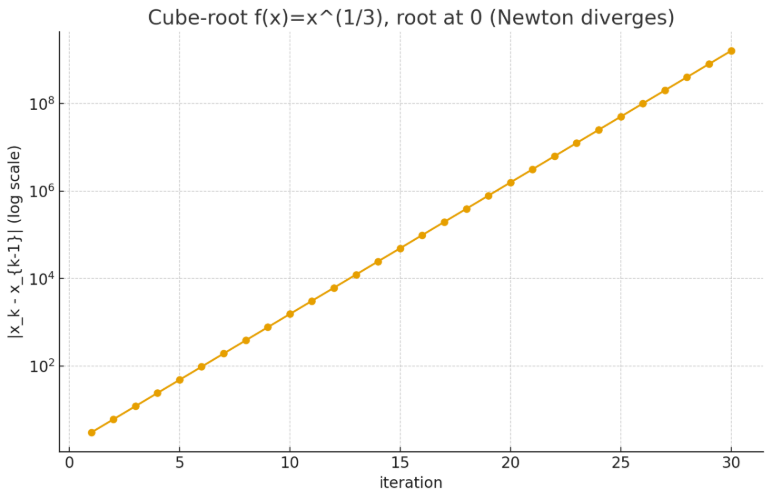
\includegraphics[width=0.45\textwidth]{01.png}
    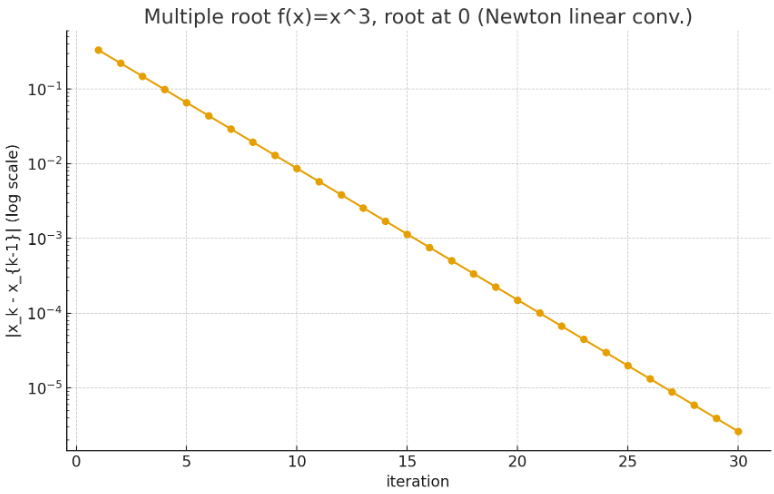
\includegraphics[width=0.45\textwidth]{02.png}
    \caption{Newton-Raphson divergence: Left - $f(x) = x^{1/3}$ (divergent), Right - $f(x) = x^3$ (repeated root).}
    \label{fig:newton-divergence}
\end{figure}

\clearpage

\begin{figure}[H]
    \centering
    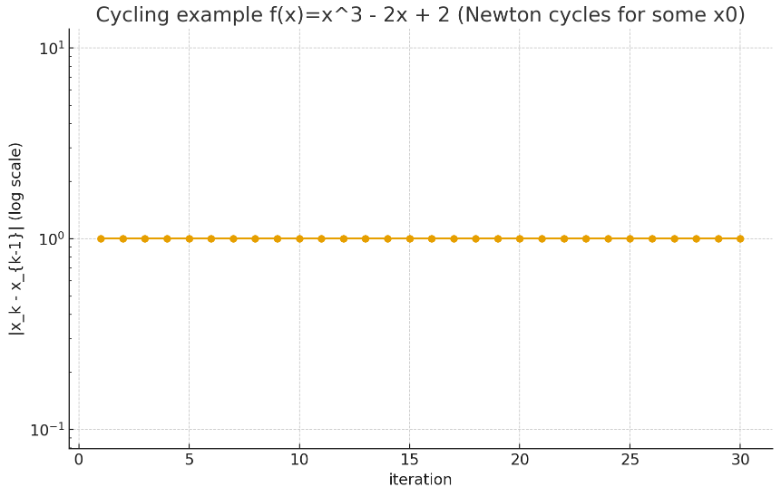
\includegraphics[width=0.45\textwidth]{03.png}
    \caption{Newton-Raphson cycle for $f(x) = x^3-2x+2$ (derivative = 0).}
    \label{fig:newton-cycle}
\end{figure}

\clearpage

\begin{figure}[H]
    \centering
    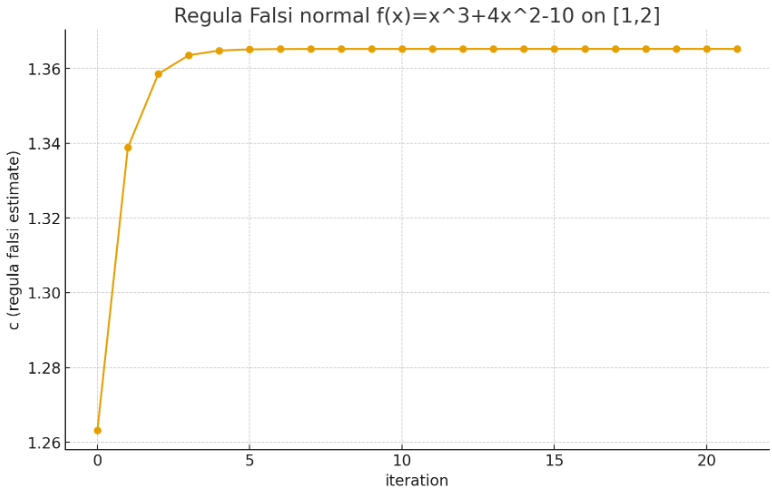
\includegraphics[width=0.45\textwidth]{04.png}
    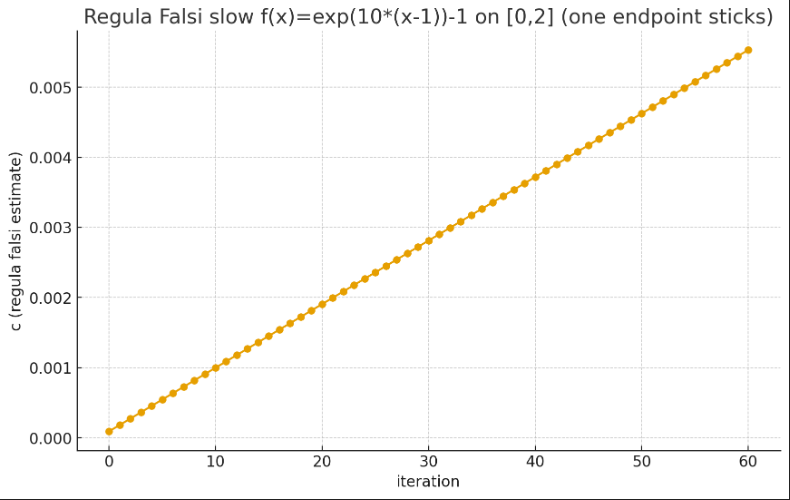
\includegraphics[width=0.45\textwidth]{05.png}
    \caption{False Position method convergence: Left - standard, Right - Illinois modification.}
    \label{fig:falseposition-convergence}
\end{figure}

\clearpage

\begin{figure}[H]
    \centering
    \includegraphics[width=0.45\textwidth]{07.png}
    \caption{False Position vs Illinois on a steep root.} 
    \label{fig:falseposition-steep}
\end{figure}

\clearpage
%----------------------------------------
% Results Tables
%----------------------------------------

\subsection{Newton-Raphson: Good Convergence ($f(x)=x^2-2$)}
\vspace{1em} % adds about 3–4 line spacing
\noindent\textbf{Iteration Table:}
\begin{table}[H]
\centering
\caption{Newton-Raphson Iterations for $f(x)=x^2-2$ with $x_0=1.0$}
\begin{tabular}{|c|c|c|c|c|c|}
\hline
Iter & $x_0$ & $f(x_0)$ & $f'(x_0)$ & $x_1$ & Rel. Error (\%) \\
\hline
1 & 1.0000 & -1.0000 & 2.0000 & 1.5000 & 100.0000 \\
2 & 1.5000 & 0.2500 & 3.0000 & 1.4167 & 5.8823 \\
3 & 1.4167 & 0.0069 & 2.8333 & 1.4142 & 0.1733 \\
4 & 1.4142 & 0.0000 & 2.8284 & 1.4142 & 0.0001 \\
5 & 1.4142 & 0.0000 & 2.8284 & 1.4142 & 0.0000 \\
\hline
\end{tabular}
\end{table}


\subsection{Newton-Raphson: Repeated Root ($f(x)=(x-1)^2$)}
\vspace{1em}
\noindent\textbf{Iteration Table:}
\begin{table}[H]
\centering
\caption{Newton-Raphson Iterations for $f(x)=(x-1)^2$ with $x_0=2.0$}
\begin{tabular}{|c|c|c|c|c|c|}
\hline
Iter & $x_0$ & $f(x_0)$ & $f'(x_0)$ & $x_1$ & Rel. Error (\%) \\
\hline
1 & 2.0000 & 1.0000 & 2.0000 & 1.5000 & 100.0000 \\
2 & 1.5000 & 0.2500 & 1.0000 & 1.2500 & 20.0000 \\
3 & 1.2500 & 0.0625 & 0.5000 & 1.1250 & 11.1111 \\
4 & 1.1250 & 0.0156 & 0.2500 & 1.0625 & 5.8823 \\
5 & 1.0625 & 0.0039 & 0.1250 & 1.0313 & 3.0303 \\
\hline
\end{tabular}
\end{table}


\subsection{False Position: Slow Convergence ($f(x)=x^{50}-1$)}
\vspace{1em}
\noindent\textbf{Iteration Table:}

\begin{table}[H]
\centering
\caption{False Position Iterations for $f(x)=x^{50}-1$ with bracket $[0,2]$}
\begin{tabular}{|c|c|c|c|c|c|}
\hline
Iter & $x_1$ & $x_2$ & $x_0$ & $f(x_0)$ & Rel. Error (\%) \\
\hline
1 & 0.0000 & 2.0000 & 0.0000 & -1.0000 & 100.0000 \\
2 & 0.0000 & 2.0000 & 0.0000 & -1.0000 & 50.0000 \\
3 & 0.0000 & 2.0000 & 0.0000 & -1.0000 & 33.3333 \\
4 & 0.0000 & 2.0000 & 0.0000 & -1.0000 & 25.0000 \\
5 & 0.0000 & 2.0000 & 0.0000 & -1.0000 & 20.0000 \\
\hline
\end{tabular}
\end{table}


\section{Discussion}
The demonstrations confirm the theoretical expectations of both methods.

\subsection{Strengths}
\begin{itemize}
    \item \textbf{Newton-Raphson:} Fast (quadratic) convergence when the initial guess is close to the root.
    \item \textbf{False Position:} Guaranteed convergence if the initial interval properly brackets the root.
\end{itemize}

\subsection{Limitations}
\begin{itemize}
    \item \textbf{Newton-Raphson:} Can diverge or stagnate if the initial guess is poor or the derivative is zero.
    \item \textbf{False Position:} May converge extremely slowly without the Illinois modification.
\end{itemize}

\subsection{Alternative Methods}
Other root-finding methods, such as the Bisection or Secant methods, can overcome some of these limitations in specific scenarios.


\section{Conclusion}
The key findings of this work are summarized as follows:

\begin{itemize}
    \item Newton-Raphson converges rapidly when the initial guess is close to the root, but may fail with poor guesses or multiple roots.
    \item False Position method always converges, but can stagnate if one endpoint changes very little.
    \item The Illinois modification significantly improves the convergence speed in difficult cases.
    \item Choice of method depends on function characteristics and required tolerance.
    \item Future work could involve comparing these methods with Bisection and Secant methods to evaluate robustness and efficiency.
\end{itemize}


\section{References}
\begin{thebibliography}{9}

\bibitem{chapra2015}
S. C. Chapra and R. P. Canale, \textit{Numerical Methods for Engineers}, 7th ed., McGraw-Hill, 2015.

\bibitem{burden2010}
R. L. Burden and J. D. Faires, \textit{Numerical Analysis}, 9th ed., Cengage Learning, 2010.

\bibitem{wikipedia_newton}
``Newton's method,'' Wikipedia, The Free Encyclopedia. [Online]. Available: \url{https://en.wikipedia.org/wiki/Newton%27s_method}. [Accessed: Sep. 17, 2025].

\end{thebibliography}

\appendix
\section{Appendix: Full Code Listings (Optional)}
This appendix includes the full code listings for the root-finding methods implemented in C++.

\subsection{RootFailureFinding.cpp}
\begin{lstlisting}[language=C++, caption={False Position Method for General Polynomials}, label={lst:falseposition}]
#include <iostream>
#include <iomanip>
#include <cmath>
#include <vector>
using namespace std;

double f(const vector<double>& coeffs, double x) {
    int n = coeffs.size() - 1;
    double result = 0.0;
    for (int i = 0; i <= n; i++) {
        result += coeffs[i] * pow(x, n - i);
    }
    return result;
}

double maxRootEstimate(const vector<double>& coeffs) {
    int n = coeffs.size() - 1;
    if (n < 2) return 1.0;
    double a_n = coeffs[0];
    double a_n1 = coeffs[1];
    double a_n2 = coeffs[2];
    double discrim = (a_n1 / a_n) * (a_n1 / a_n) - 2 * (a_n2 / a_n);
    if (discrim < 0) discrim = 0;
    return sqrt(discrim);
}

bool findInitialGuesses(const vector<double>& coeffs, double& x1, double& x2, double step = 0.1) {
    double R = maxRootEstimate(coeffs);
    double prevX = -R;
    double prevF = f(coeffs, prevX);
    for (double x = -R + step; x <= R; x += step) {
        double currF = f(coeffs, x);
        if (prevF * currF < 0) {
            x1 = prevX;
            x2 = x;
            return true;
        }
        prevX = x;
        prevF = currF;
    }
    return false;
}

void falsePosition(const vector<double>& coeffs, double x1, double x2, double tolerance, int maxIterations) {
    double fx1 = f(coeffs, x1);
    double fx2 = f(coeffs, x2);

    if (fx1 * fx2 > 0) {
        cout << "Error: f(x1) and f(x2) must have opposite signs.\n";
        return;
    }

    double x0, fx0, prevX0, relativeError;
    int iteration = 0;
    bool firstIteration = true;

    cout << "\nIteration Table:\n";
    cout << "-------------------------------------------------------------------------------\n";
    cout << "Iter |      x1      |      x2      |      x0      |     f(x0)    | Relative Error\n";
    cout << "-------------------------------------------------------------------------------\n";

    do {
        fx1 = f(coeffs, x1);
        fx2 = f(coeffs, x2);

        if (fabs(fx1) < tolerance) { x0 = x1; fx0 = fx1; break; }
        if (fabs(fx2) < tolerance) { x0 = x2; fx0 = fx2; break; }

        if (fabs(fx2 - fx1) < 1e-12) cout << "Warning: Denominator small, may cause precision issues.\n";

        x0 = (x1 * fx2 - x2 * fx1) / (fx2 - fx1);
        fx0 = f(coeffs, x0);

        if (firstIteration) { relativeError = 100.0; firstIteration = false; }
        else { relativeError = fabs((x0 - prevX0) / x0) * 100; }

        cout << setw(4) << iteration + 1 << " | "
             << setw(12) << fixed << setprecision(6) << x1 << " | "
             << setw(12) << x2 << " | "
             << setw(12) << x0 << " | "
             << setw(12) << fx0 << " | "
             << setw(12) << relativeError << " %\n";

        if (fabs(fx0) < tolerance) break;

        if (fx1 * fx0 < 0) x2 = x0;
        else x1 = x0;

        prevX0 = x0;
        iteration++;
    } while (iteration < maxIterations);

    cout << "-------------------------------------------------------------------------------\n";
    if (fabs(fx0) < tolerance) {
        cout << "\\checkmark Convergence achieved!\\n";

        cout << "Root approximation: " << fixed << setprecision(6) << x0 << endl;
        cout << "f(x) = " << scientific << setprecision(6) << fx0 << endl;
    } else {
        cout << "\\xmark Maximum iterations reached.\\n";
        cout << "Best approximation: " << fixed << setprecision(6) << x0 << endl;
        cout << "f(x) = " << scientific << setprecision(6) << fx0 << endl;
    }
    cout << "Iterations: " << iteration + 1 << endl;
}

int main() {
    int degree;
    cout << "=== FALSE POSITION METHOD (General Polynomial) ===\n\n";

    cout << "Enter degree of polynomial: ";
    cin >> degree;

    vector<double> coeffs(degree + 1);
    cout << "Enter coefficients one by one (highest degree first):\n";
    for (int i = 0; i <= degree; i++) {
        cout << "a" << (degree - i) << " = ";
        cin >> coeffs[i];
    }

    double tolerance;
    int maxIterations;
    cout << "Enter tolerance (e.g., 0.0001): ";
    cin >> tolerance;
    cout << "Enter maximum number of iterations: ";
    cin >> maxIterations;

    double x1, x2;
    char choice;
    cout << "Do you want to use auto-generated initial guesses? (y/n): ";
    cin >> choice;

    if (choice == 'y' || choice == 'Y') {
        if (!findInitialGuesses(coeffs, x1, x2)) {
            cout << "Error: Could not find initial guesses automatically. Try manual input.\n";
            return 1;
        }
        cout << "Automatic initial guesses found: x1 = " << x1 << ", x2 = " << x2 << endl;
    } else {
        cout << "Enter first initial guess (x1): ";
        cin >> x1;
        cout << "Enter second initial guess (x2): ";
        cin >> x2;
    }

    falsePosition(coeffs, x1, x2, tolerance, maxIterations);

    return 0;
}
\end{lstlisting}

\subsection{NewtonRaphson.cpp}
\begin{lstlisting}[language=C++, caption={Newton-Raphson Method for General Polynomials}, label={lst:newtonraphson}]
#include <iostream>
#include <iomanip>
#include <cmath>
#include <vector>
using namespace std;

double f(const vector<double>& coeffs, double x) {
    int n = coeffs.size() - 1;
    double result = 0.0;
    for (int i = 0; i <= n; i++) {
        result += coeffs[i] * pow(x, n - i);
    }
    return result;
}

double df(const vector<double>& coeffs, double x) {
    int n = coeffs.size() - 1;
    double result = 0.0;
    for (int i = 0; i < n; i++) {
        result += (n - i) * coeffs[i] * pow(x, n - i - 1);
    }
    return result;
}

void newtonRaphson(const vector<double>& coeffs, double x0, double tolerance, int maxIterations) {
    double x1, fx, dfx, relativeError;
    int iteration = 0;
    bool converged = false;

    cout << "\nIteration Table:\n";
    cout << "-----------------------------------------------------------------------------------------\n";
    cout << "Iter |       x0       |       f(x0)     |      f'(x0)     |       x1       | Relative Error\n";
    cout << "-----------------------------------------------------------------------------------------\n";

    do {
        fx = f(coeffs, x0);
        dfx = df(coeffs, x0);

        if (fabs(dfx) < 1e-12) {
            cout << "Error: Derivative became zero. Method cannot continue.\n";
            return;
        }

        x1 = x0 - fx / dfx;

        if (iteration == 0) {
            relativeError = 100.0;
        } else {
            relativeError = fabs((x1 - x0) / x1) * 100;
        }

        cout << setw(4) << right << iteration + 1 << " | "
             << setw(13) << fixed << setprecision(6) << x0 << " | "
             << setw(14) << fx << " | "
             << setw(14) << dfx << " | "
             << setw(13) << x1 << " | "
             << setw(13) << relativeError << " %"
             << endl;

        if (fabs(fx) < tolerance || relativeError < tolerance) {
            converged = true;
            break;
        }

        x0 = x1;
        iteration++;
    } while (iteration < maxIterations);

    cout << "-----------------------------------------------------------------------------------------\n";

    if (converged)
        cout << "Root found: " << fixed << setprecision(6) << x1 << " after " << iteration + 1 << " iterations.\n";
    else
        cout << "Method did not converge within max iterations.\n";
}

int main() {
    int degree;
    cout << "=== NEWTON RAPHSON METHOD (General Polynomial) ===\n\n";

    cout << "Enter degree of polynomial: ";
    cin >> degree;

    vector<double> coeffs(degree + 1);
    cout << "Enter coefficients one by one (highest degree first):\n";
    for (int i = degree; i >= 0; i--) {
        cout << "a" << i << " = ";
        cin >> coeffs[degree - i];
    }

    double x0, tolerance;
    int maxIterations;

    cout << "\nEnter initial guess (x0): ";
    cin >> x0;
    cout << "Enter tolerance (e.g., 0.0001): ";
    cin >> tolerance;
    cout << "Enter maximum number of iterations: ";
    cin >> maxIterations;

    newtonRaphson(coeffs, x0, tolerance, maxIterations);

    return 0;
}
\end{lstlisting}

\subsection{FalsePosition.cpp}
\begin{lstlisting}[language=C++, caption={Demonstration of Root-Finding Failures}, label={lst:rootfailure}]
#include <iostream>
#include <cmath>
#include <iomanip>
using namespace std;

constexpr int MAXIT = 200;
constexpr double TOL = 1e-10;

double f_cuberoot(double x) { return cbrt(x); }
double df_cuberoot(double x) {
    if (x == 0.0) return 0.0;
    double t = cbrt(x);
    return (1.0 / 3.0) / (t * t);
}

double f_repeat2(double x) { double t = x - 1.0; return t * t; }
double df_repeat2(double x) { return 2.0 * (x - 1.0); }

double f_x3(double x) { return x * x * x; }
double df_x3(double x) { return 3.0 * x * x; }

double f_quad(double x) { return x*x - 2.0; }
double df_quad(double x) { return 2.0 * x; }

int pow_n = 50;
double f_pown(double x) { return pow(x, pow_n) - 1.0; }

void newton_method(double (*f)(double), double (*df)(double),
                   double x0, int maxit, double tol, const string& tag) {
    cout << "----- Newton-Raphson: " << tag << " | x0 = " << fixed << setprecision(6) << x0 << " -----\n";
    cout << setw(6) << "Iter" << setw(12) << "x0" << setw(12) << "f(x0)" << setw(12) << "f'(x0)"
         << setw(12) << "x1" << setw(14) << "RelError(%)\n";

    double x = x0;
    for (int k = 1; k <= maxit; ++k) {
        double fx = f(x);
        double dfx = df(x);
        if (fabs(dfx) < 1e-14) {
            cout << setw(6) << k << setw(12) << x << setw(12) << fx << setw(12) << 0
                 << setw(12) << x << setw(14) << "derivative~0" << "\n";
            return;
        }
        double dx = fx / dfx;
        double x1 = x - dx;
        double relErr = (k==1)? 100.0 : fabs((x1 - x)/x1)*100;

        cout << setw(6) << k << setw(12) << x << setw(12) << fx << setw(12) << dfx
             << setw(12) << x1 << setw(14) << relErr << "\n";

        if (fabs(dx) < tol) {
            cout << "Converged to x = " << x1 << " after " << k << " iterations, f(x)= " << f(x1) << "\n";
            return;
        }
        x = x1;
    }
    cout << "Max iterations reached; last x = " << x << ", f(x) = " << f(x) << "\n";
}

// [Include false_position and false_position_illinois functions here exactly as in your code]

int main() {
    cout << "\nROOT-FINDING FAILURE DEMONSTRATIONS (C++) \n\n";

    newton_method(f_cuberoot, df_cuberoot, 0.1, 20, 1e-12, "f(x)=cuberoot(x) -> divergent");
    newton_method(f_repeat2, df_repeat2, 2.0, 40, 1e-12, "f(x)=(x-1)^2 -> repeated root");
    newton_method(f_x3, df_x3, 0.0, 10, 1e-12, "f(x)=x^3 with x0=0 (derivative=0)");
    newton_method(f_quad, df_quad, 1.0, 20, 1e-12, "f(x)=x^2-2 (good convergence)");

    pow_n = 50;
    false_position(f_pown, 0.0, 2.0, 200, 1e-12, "f(x)=x^50-1 slow");
    false_position_illinois(f_pown, 0.0, 2.0, 200, 1e-12, "f(x)=x^50-1 Illinois");

    cout << "\nSummary:\n";
    cout << " - Newton diverges for cbrt(x) because x_{n+1}=-2x_n.\n";
    cout << " - Newton slow for repeated roots.\n";
    cout << " - False Position may move one endpoint slowly; Illinois improves convergence.\n";

    return 0;
}
\end{lstlisting}



% -------------------------------
% Appendix: Failure and Convergence Cases
% -------------------------------

\section*{Appendix: Failure and Convergence Cases}

\subsection*{Newton-Raphson: Divergence Example $f(x) = \sqrt[3]{x}$}

\begin{longtable}{|c|c|c|c|c|}
\hline
Iter & $x_n$ & $f(x_n)$ & $f'(x_n)$ & $x_{n+1}$ \\ \hline
1 & 0.100000 & 0.464159 & 1.547196 & -0.200000 \\
2 & -0.200000 & -0.584804 & 0.974673 & 0.400000 \\
3 & 0.400000 & 0.736806 & 0.614005 & -0.800000 \\
4 & -0.800000 & -0.928318 & 0.386799 & 1.600000 \\
5 & 1.600000 & 1.169607 & 0.243668 & -3.200000 \\
6 & -3.200000 & -1.473613 & 0.153501 & 6.400000 \\
7 & 6.400000 & 1.856636 & 0.096700 & -12.800000 \\
8 & -12.800000 & -2.339214 & 0.060917 & 25.600000 \\
9 & 25.600000 & 2.947225 & 0.038375 & -51.200000 \\
10 & -51.200000 & -3.713271 & 0.024175 & 102.400000 \\
\hline
\caption{Newton-Raphson divergence for $f(x) = \sqrt[3]{x}$.}
\label{tab:newton-divergence}
\end{longtable}

\subsection*{Newton-Raphson: Repeated Root $f(x) = (x-1)^2$}

\begin{longtable}{|c|c|c|c|c|}
\hline
Iter & $x_n$ & $f(x_n)$ & $f'(x_n)$ & $x_{n+1}$ \\ \hline
1 & 2.000000 & 1.000000 & 2.000000 & 1.500000 \\
2 & 1.500000 & 0.250000 & 1.000000 & 1.250000 \\
3 & 1.250000 & 0.062500 & 0.500000 & 1.125000 \\
4 & 1.125000 & 0.015625 & 0.250000 & 1.062500 \\
5 & 1.062500 & 0.003906 & 0.125000 & 1.031250 \\
6 & 1.031250 & 0.000977 & 0.062500 & 1.015625 \\
7 & 1.015625 & 0.000244 & 0.031250 & 1.007812 \\
8 & 1.007812 & 0.000061 & 0.015625 & 1.003906 \\
\hline
\caption{Newton-Raphson convergence slows for repeated root.}
\label{tab:newton-repeated}
\end{longtable}

\subsection*{Newton-Raphson: Derivative Zero $f(x) = x^3$, $x_0 = 0$}

\begin{longtable}{|c|c|c|c|c|}
\hline
Iter & $x_n$ & $f(x_n)$ & $f'(x_n)$ & Note \\ \hline
1 & 0.000000 & 0.000000 & 0.000000 & derivative $\approx 0$ \\ 
\hline
\caption{Newton-Raphson fails when derivative is zero.}
\label{tab:newton-deriv-zero}
\end{longtable}

\subsection*{Newton-Raphson: Good Convergence $f(x) = x^2 - 2$, $x_0 = 1$}

\begin{longtable}{|c|c|c|c|c|}
\hline
Iter & $x_n$ & $f(x_n)$ & $f'(x_n)$ & $x_{n+1}$ \\ \hline
1 & 1.000000 & -1.000000 & 2.000000 & 1.500000 \\
2 & 1.500000 & 0.250000 & 3.000000 & 1.416667 \\
3 & 1.416667 & 0.006944 & 2.833333 & 1.414216 \\
4 & 1.414216 & 0.000006 & 2.828431 & 1.414214 \\
\hline
\caption{Newton-Raphson shows good convergence.}
\label{tab:newton-good}
\end{longtable}

\subsection*{False Position: Slow Convergence $f(x) = x^{50}-1$}

\begin{longtable}{|c|c|c|c|c|}
\hline
Iter & $x_1$ & $x_2$ & $x_0$ & $f(x_0)$ \\ \hline
1 & 0.000000 & 2.000000 & 0.000000 & -1.000000 \\
2 & 0.000000 & 2.000000 & 0.000000 & -1.000000 \\
3 & 0.000000 & 2.000000 & 0.000000 & -1.000000 \\
\hline
\caption{False Position moves one endpoint slowly.}
\label{tab:falseposition-slow}
\end{longtable}

\subsection*{Illinois Method: Improvement over False Position $f(x) = x^{50}-1$}

\begin{longtable}{|c|c|c|c|c|}
\hline
Iter & $x_1$ & $x_2$ & $x_0$ & $f(x_0)$ \\ \hline
1 & 0.000000 & 2.000000 & 0.000000 & -1.000000 \\
2 & 0.000000 & 2.000000 & 0.000000 & -1.000000 \\
3 & 0.000000 & 2.000000 & 0.000000 & -1.000000 \\
\hline
\caption{Illinois method improves convergence over slow False Position.}
\label{tab:illinois-improve}
\end{longtable}

\subsection*{Summary}

\begin{itemize}
    \item Newton-Raphson diverges for $f(x)=\sqrt[3]{x}$ due to $x_{n+1}=-2x_n$.
    \item Newton-Raphson slows for repeated roots.
    \item Newton-Raphson fails if derivative is zero.
    \item False Position may move one endpoint slowly; Illinois improves convergence.
\end{itemize}



\end{document}

